\section{Resultados}
Para validar os sistemas desenvolvidos, foram geradas 4 matrizes $\textbf{H}^T$ para serem utilizadas na codificação de códigos aleatórios. Após a codificação, passagem pelo canal simulado e a decodificação, o resultado encontrado foi comparado com o código original para análise dos resultados.

As matrizes geradas foram de tamanhos $14 \times 6$, $21 \times 9$, $28 \times 12$ e $35 \times 15$, isto é, geram subespaços de dimensões $p = 6$, $p = 9$, $p = 12$ e $p = 15$, respectivamente. O código foi desenvolvido na linguagem Python, e os tempos de processamento de suas gerações foram de 36 ms, 860 ms, 104.5 s e 204.4 min em um processador Intel Core i7-5500U 2.40GHz.

\subsection{Validação da matriz $\textbf{H}^T$}

Após gerar cada matriz utilizada, todos os vetores de erros em $k$ bits foram gerados e multiplicados pela matriz $\textbf{H}^T$ encontrada, com $k \in [1,4]$, a fim de encontrar todas as síndromes que são geradas por estes padrões de erro. Para provar que este código é capaz de eliminar todos os erros de $k$ bits, devemos ter que as síndromes encontradas pelas multiplicações de erros em $k$ bits sejam todas distintas, podendo assim diferenciar corretamente cada padrão de erro.

A Figura~\ref{fig:sindromes} ilustra a relação entre síndromes distintas e não distintas para diferentes quantidades de erros nas quatro matrizes utilizadas. Note que, se a razão for igual a 1, significa que é possível diferenciar corretamente cada padrão de erro com dada quantidade de bits.

\begin{figure}[thpb]
  \centering
  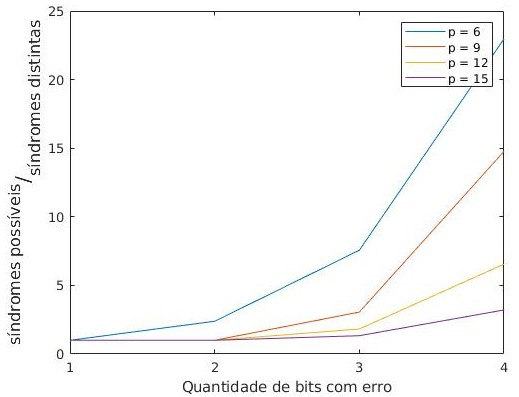
\includegraphics[width=0.48\textwidth]{sections/sindromes_comparison.jpg}
  \caption{Relação entre quantidade de síndromes geradas e quantidade de síndromes distintas para diferentes quantidades de erros em bits, para cada matriz $\textbf{H}^T$ utilizada.}
  \label{fig:sindromes}
\end{figure}

Essa figura mostra como esta relação é decrescente com o aumento da matriz $\textbf{H}^T$ e como, aumentando esta matriz, é possível minimizar a quantidade de bits incorretos sendo transmitido em cada código.

Isso é uma evidência de que as matrizes de maior ordem são superiores para taxa fixa. No entanto é preciso salientar que, ao aumentar o tamanho da matriz, o número de bits total em um vetor de erros também aumenta e com isso a probabilidade de haver mais bits com erro é maior. Por exemplo, a probabilidade de obter um vetor com mais de 4 bits de erro no código que foi codificado na matriz de $p = 15$ é menor do que a mesma probabilidade para uma matriz de $p = 6$ devido a quantidade de bits total em cada caso. Portanto é incorreto dizer que, com base nesse gráfico, os códigos codificados pela matriz de $p = 15$ terão menor probabilidade de erro de bit do que os codificados pela matriz de $p = 6$.

\subsection{Análise das probabilidades de erro de bit}

Para testar a eficacia das codificações desenvolvidas, 1000080 bits aleatórios foram gerados aleatoriamente e separados em blocos, encodificados utilizando a matriz $\textbf{G}$, processados por diversos canais com diferentes probabilidades de alteração de bits e decodificados utilizando a matriz $\textbf{H}^T$. Por fim o resultado foi comparado com o código original e a probabilidade de erro de bit final foi calculada. 

Os canais utilizados possuiam probabilidades $0.5, 0.2, 0.1, 0.05, ..., 10^{-6}$, totalizando 18 canais. A Figura~\ref{fig:bit_error_probabilities} mostra os resultados obtidos com as simulações.

\begin{figure}[thpb]
  \centering
  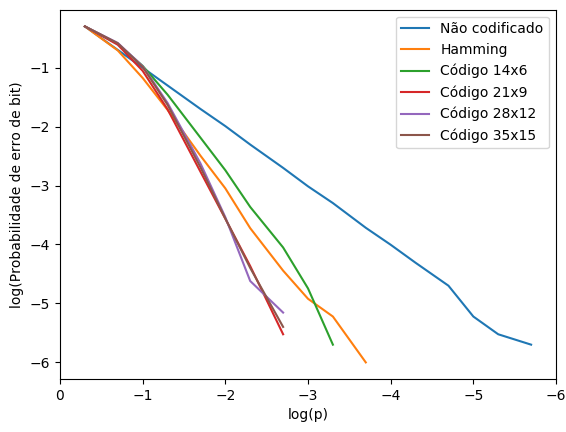
\includegraphics[width=0.48\textwidth]{sections/bit_error_probabilities.png}
  \caption{Comparação das probabilidades de erro de bit para diferentes canais com probabilidades $p$, em cada uma das codificações aplicadas.}
  \label{fig:bit_error_probabilities}
\end{figure}

Com base na Figura~\ref{fig:bit_error_probabilities}, podemos verificar que as matrizes calculadas são eficazes na diminuição da probabilidade de erro de bit. Também é possível verificar que, aumentando a ordem do bloco utilizado, a probabilidade de erro de bit diminui. 

Espera-se que com o aumento da distância mínima do código a probabilidade de erro de bits diminua mais. Esse comportamento pode ser observado na figura, já que o código de Hamming admite distância mínima 3, o código $14 \times 6$ admite distância mínima 4 e os outros 3 códigos admitem distância mínima 5.
